\section{系统架构}
\label{sec:system_architecture}

\subsection{总体架构设计}
系统采用“主系统 + 插件执行端 + 数据资源层 + 智能解析服务 + 仿真分析模块”的分层协作结构。这样设计的原因在于：用户交互、任务理解、三维执行、数据存储和动态展示的变化频率并不一致，将它们拆开能够减少耦合，并方便后续单独扩展模型服务、插件能力或资源类型。

\begin{table}[t]
\centering
\caption{高层子系统职责划分}
\label{tab:subsystem_responsibilities}
\rowcolors{2}{gray!8}{white}
\begin{tabularx}{\textwidth}{p{3.2cm} Y}
\rowcolor{gray!20}
\toprule
子系统 & 核心职责 \\
\midrule
用户工作台 & 提供登录、项目浏览、参数配置、任务确认、结果查看和导出交互 \\
任务调度 & 接收输入、校验权限、封装任务、分发执行、跟踪状态与回写结果 \\
LLM 解析 & 将自然语言、草图摘要和上下文解析为结构化任务建议 \\
Blender 插件适配 & 接收结构化任务并完成建模、替换、布局更新和场景保存 \\
资源与项目数据 & 保存项目、场景、资产、布局数据、任务记录与日志数据 \\
动态仿真 & 在生成后的场景上配置车辆、人群和船只等动态展示效果 \\
后台治理 & 管理用户、角色、权限、插件状态、模型服务和审计日志 \\
\bottomrule
\end{tabularx}
\end{table}

\subsection{分层关系说明}
\begin{enumerate}[label=\arabic*.]
    \item 表现层：由建模师工作台、分析师工作台和管理员工作台组成，负责输入和展示。
    \item 应用层：由任务调度、项目管理、版本管理、权限控制等服务组成，负责流程编排。
    \item 领域层：由场景、布局、任务、资产、仿真和日志等核心领域对象组成，负责表达业务语义。
    \item 基础设施层：由 Blender 插件接口、数据库、文件存储、模型服务接口组成，负责外部依赖接入。
\end{enumerate}

\subsection{模块分解说明}
\subsubsection*{1. 系统整体结构分解}

图~\ref{fig:system_overview}描述了系统在高层视角下的整体结构。系统首先划分为统一登录与身份认证入口，以及面向不同角色的三个工作台：场景建模师工作台、行业分析师工作台和系统管理员工作台。建模师工作台负责场景创建、布局调整、插件调用和结果修订；分析师工作台负责场景查看、动态仿真、方案比较与结果导出；管理员工作台负责用户管理、权限配置、模型服务维护和日志审计。

在角色工作台之外，系统还进一步分解出结果与治理相关的公共支撑部分，包括项目结果管理、版本留存和日志记录。三个工作台在完成各自任务后，均需要与这些公共支撑部分发生交互，以保证系统具备结果保存、版本回溯和行为追踪能力。由此形成的高层结构说明，本系统不是单一建模工具，而是由统一入口、角色工作台和公共支撑模块共同组成的协同系统。

\subsubsection*{2. 系统数据与任务流分解}
\begin{figure}[H]
\centering
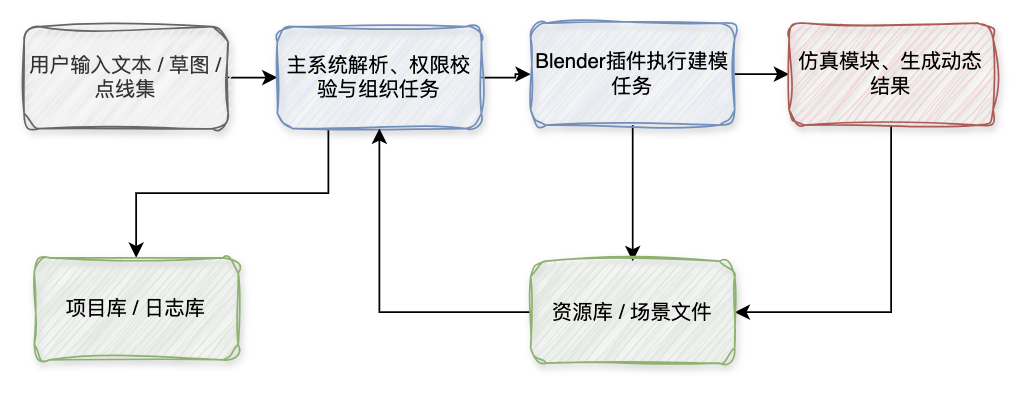
\includegraphics[width=\textwidth]{figures/8.png}
\caption{系统数据与任务流分解图}
\label{fig:architecture_data_flow}
\end{figure}

图~\ref{fig:architecture_data_flow}反映了系统在执行链路上的组成方式。按照任务流和数据流关系，系统可分解为主系统、Blender 插件、资产库、场景文件、仿真模块、项目库和日志库。主系统负责接收用户输入并完成权限判断、输入规范化、参数补全和任务封装；Blender 插件负责执行具体生成与修改任务；资产库和场景文件为插件执行提供资源与场景上下文；仿真模块负责在生成结果基础上补充动态展示；项目库和日志库分别负责结果版本保存与执行过程留痕。

这些部分之间通过统一任务链路衔接：输入先进入主系统，任务由主系统下发至 Blender 插件，执行结果回流至主系统并同步写入项目库和日志库，涉及动态对象时再继续流入仿真模块。由此形成的分解结果明确了各子系统在执行链路中的职责边界，也明确了任务、结果和日志在系统中的回写路径。

\subsubsection*{3. 系统功能结构分解}
\begin{figure}[H]
\centering
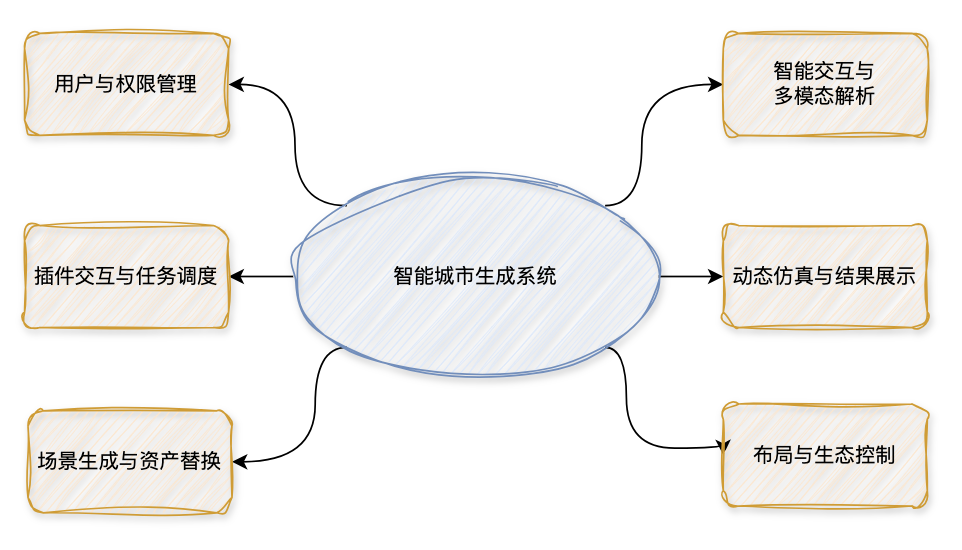
\includegraphics[width=\textwidth]{figures/9.png}
\caption{系统功能结构分解图}
\label{fig:function_structure}
\end{figure}

图~\ref{fig:function_structure}从功能视角展示了系统的模块划分。根据需求边界与职责划分，系统功能可分解为六个核心模块：用户与权限管理、插件交互与任务调度、场景生成与资产替换、布局与生态控制、智能交互与多模态解析、动态仿真与结果展示。其中，用户与权限管理负责系统入口控制与后台治理；插件交互与任务调度负责连接主系统与 Blender 执行端；场景生成与资产替换负责基础城市场景构建与对象替换；布局与生态控制负责空间结构调整与生态对象生成；智能交互与多模态解析负责自然语言、草图和参数表单的统一理解；动态仿真与结果展示负责车辆、人群、船只等动态效果呈现与结果导出。

在此基础上，各模块之间形成清晰的协作关系：权限模块提供访问边界，任务调度模块组织执行链路，场景生成与布局控制模块承担主要建模能力，智能交互模块负责把用户意图转化为可执行任务，动态仿真模块负责补充结果展示。这样的分解结果使系统后续能够围绕模块边界开展接口定义、对象划分和实现分工。

\subsection{架构决策说明}
\begin{enumerate}[label=\arabic*.]
    \item 不让 LLM 直接操作 Blender，而是先生成结构化任务，以保证执行可控。
    \item 不让场景结果只保留最终态，而是保留项目和场景版本，支撑回滚与比较。
    \item 不将仿真逻辑与基础建模强耦合，便于只做静态生成或后续升级动态能力。
    \item 不让管理员直接介入建模链路，而是通过治理模块进行用户、资源和服务维护。
\end{enumerate}
